\section*{Agreement with LD Score regression}

Both reports lean on cross-trait LDSC as the independent check on the joint
fit, so it is worth showing what that check actually looks like across every
pair rather than quoting it one pair at a time.

Three further pairs are drawn in from \texttt{benchmarks/qc\_factorial.csv} at
the same arm 001 --- LDL $\times$ CAD, height $\times$ LDL and HDL $\times$ TG.
They extend the range in both directions: HDL $\times$ TG is the only strongly
negative \texttt{rg} available, and height is the most heritable trait in
either set. They are marked with triangles because they come from a different
script and a separately screened variant set; the factorial's LDL $\times$ CAD
retains 832{,}668 variants where the \texttt{ldl-cad} study retains 845{,}623,
so the two are close but not the same fit.

\begin{figure}[H]
\centering
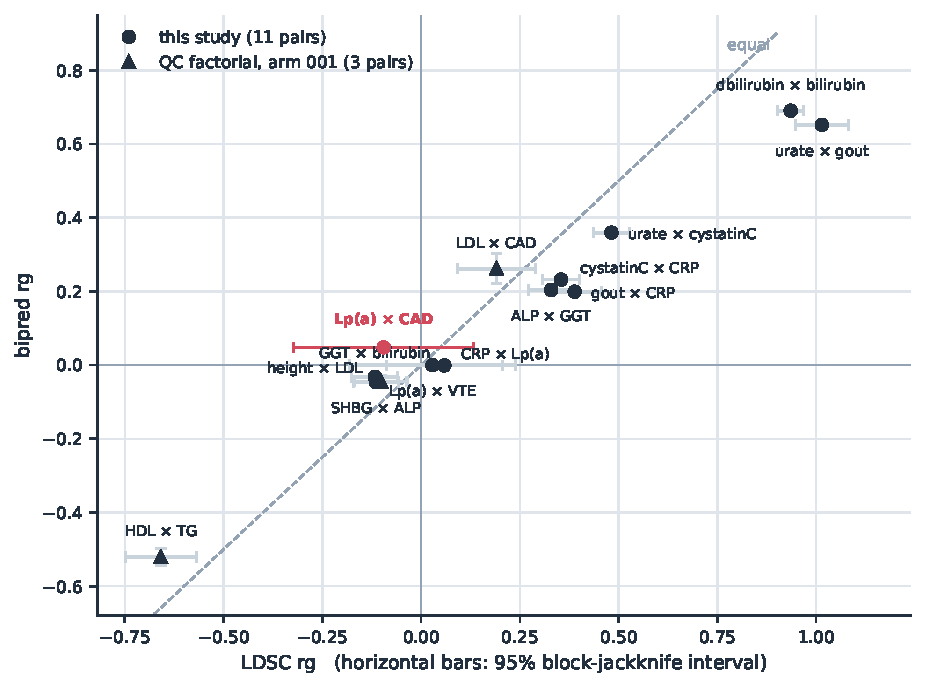
\includegraphics[width=\linewidth]{figures/rg-agreement.pdf}
\caption{bipred \texttt{rg} against cross-trait LDSC \texttt{rg}. The two agree
on sign and ordering across the full range, from $-0.66$ to $+1.01$. They do
not agree on magnitude: bipred is consistently pulled toward zero at both ends
--- $+0.65$ against LDSC's $+1.01$ for urate $\times$ gout, $-0.52$ against
$-0.66$ for HDL $\times$ TG. Lp(a) $\times$ CAD is the pair where they disagree
in sign, and it is also the pair with the widest LDSC interval: the jackknife
bar runs from $-0.32$ to $+0.13$, so LDSC is not resolving this pair at all.}
\end{figure}

That last point is worth separating from the study's main claim. The reason to
prefer \texttt{rho\_beta} for Lp(a) $\times$ CAD is not that LDSC gives a
different answer --- LDSC gives an answer with an interval four times wider
than the estimate, which is what a genome-wide average does on a trait with
$\sim$100 causal variants.

\begin{figure}[H]
\centering
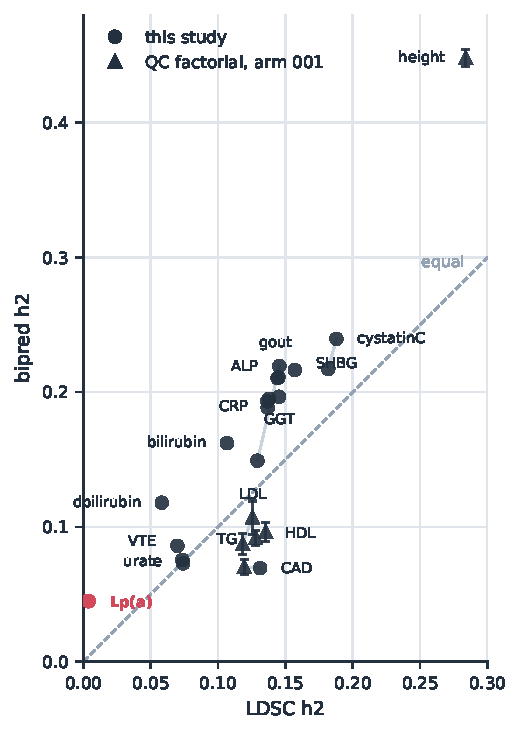
\includegraphics[width=\linewidth]{figures/h2-agreement.pdf}
\caption{Per-trait \texttt{h2}, both estimators, log scale. Points are one
trait in one pairing, joined where a trait appears more than once; the joins
are therefore an empirical stability check, and most are short. The two
estimators track each other over two orders of magnitude, with bipred running
slightly high through the middle of the range. Three disagreements stand out:
CAD ($0.13 \rightarrow 0.07$) and urate ($0.07 \rightarrow 0.05$), where bipred
is lower, and height ($0.28 \rightarrow 0.43$), where it is much higher.}
\end{figure}

The joins also expose one instability worth recording. Gout moves from
\texttt{h2} $0.11$ in urate $\times$ gout to $0.21$ in gout $\times$ CRP, an
86\% change, while LDSC moves $0.13 \rightarrow 0.15$ over the same two fits.
The variant sets differ between pairs, since the screen masks are intersected
per pair, but that is a 3\% difference in $m$ against a doubling in
\texttt{h2}. No other trait behaves this way.

\subsection*{What is missing here}

Only one of the four quantities plotted above has an interval, and it is
LDSC's. That is a recording gap rather than a methodological one:

\begin{itemize}\setlength{\itemsep}{0.3em}
\item \textbf{LDSC \texttt{rg}} --- block-jackknife standard error, recorded
  everywhere. These are the horizontal bars.
\item \textbf{bipred \texttt{rg} and \texttt{h2}} --- the factorial records an
  iterate SD, the vertical bars on the three triangles. This study's CSV records
  none. Note what the factorial's bars measure: spread across retained Gibbs
  iterates, which is Monte-Carlo variability of the fit and not sampling error
  of the GWAS. At around 1\% of \texttt{h2} they are far too narrow to read as
  confidence intervals.
\item \textbf{LDSC \texttt{h2}} --- no standard error at all.
  \texttt{LDSCRgResult} returns \texttt{h2} as a bare tuple.
\end{itemize}

\texttt{BivariateResult} retains \texttt{genetic\_samples}, the raw
$(\mathrm{gvar}_1, \mathrm{gcov}, \mathrm{gvar}_2)$ quadratics at every
post-burn-in sweep, so posterior spread for both \texttt{h2} and \texttt{rg} is
recoverable from a fit --- the drivers simply do not summarise it into the CSV.
Recording those percentiles, and a jackknife standard error for LDSC
\texttt{h2}, is the change that would let this section carry real intervals.
Until then the bars above should be read as what they are.
